\chapter{Introduction}
\label{chap:intro}

\section{Hash Functions}

A hash function $H:\{0,1\}^* \rightarrow \{0,1\}^n $ is a deterministic function which compresses an input of arbitrary size to a fixed size output. The cryptographic applications of a hash function further require it to satisfy the following conditions.

\begin{itemize}\setlength\itemindent{20pt}
    \item Efficient : Given $m$, it is easy to compute $H(m)$.
    \item Preimage Resistance : Given $H(m)$, it is computationally hard to find $m$.
    \item Second-preimage Resistance : Given $m$, it is computationally hard to find $m^\prime$ such that $H(m)=H(m^\prime)$.
    \item Collision Resistance : It is computationally hard to find $m$ and $m^\prime$ such that $H(m)=H(m^\prime)$.
\end{itemize}

The hash function having the above properties are referred as cryptographic hash functions. Cryptographic hash functions are an important component of modern cryptography. These are one way functions with a mathematical function which is computationally hard to invert. The input of such a function is generally called a message i.e. $m$ and the output i.e. $H(m)$ is often referred as digest or fingerprint of the message $m$.

\section{Some Applications of Hash functions}

So a hash function maps data of any size to a data of fixed size. Due to the above listed properties hash functions have found many applications in the field of computer science. A few very basic applications of hash functions are :
\begin{enumerate}
	\item Creating a digest from the message and then using the digest later to ensure that there are no changes to the message. This property is called message integrity. Hash functions are widely used for the verification of message integrity.
	\item Hash functions are also used for storing passwords. Secure applications don't actually store the passwords directly in the database but the hash of the password is stored in the database by using a secure hash function for calculating hash. The hash stored in the database is used in future for comparing with the hash of the password entered by the user and then appropriate action is taken on a successful match. In case of a security breach the attacker knows only the hashes stored in the database not the actual passwords. Deriving password (Preimage) from the hash is again a computationally hard problem.
\end{enumerate}

Hash function is an integral component of cryptography. It is used in many cryptographic applications e.g., Authentication, Non-repudiation, Digital Signatures and Integrity etc..

\section{History of Hash functions}

There are many popular families of hash functions like MD (Message Digest) and \SHA(Secure Hash Algorithm). The MD family of hash functions comprises of MD4, MD5 etc.. Similarly \SHA{} family of hash functions comprises of \SHA-0, \SHA-1, \SHA-2, and \SHA-3.
Though \SHA-3 belongs to the same family as \SHA-2, yet it has a different structure and construction.

Most of these popular hash functions like MD5, \SHA-2 follow the Merkle-Damgard construction~\cite{merkle}. As seen in figure:~\ref{MDConstruction}.

\begin{figure}
    \centering
    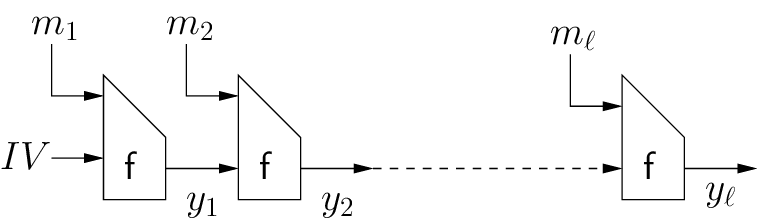
\includegraphics[scale=0.5]{MDConstruction.png}
    \caption{Merkle Damgard Construction~\cite{MDamgard}}
    \label{MDConstruction}
\end{figure}

So, how does a Hash function compress data of arbitrary any size to a fixed length output. In this construction it uses a compression function \textbf{f} which takes as input a fixed-length data and generates a data of fixed-length $n$ which is shorter than length of input data. If the input size $b$ is greater than $n$, then the function \textbf{f} accepts two inputs such that it is of the form $\big\{0,1\big\}^n \times \big\{0,1\big\}^{b - n} \rightarrow \big\{0,1\big\}^n$. To hash a message $M$ of size $N$ bits, it is divided into message blocks of size $b-n$ i.e. block size and then each block is processed by \textbf{f} one by one in the order the message is broken into blocks. So a hash function $H$ just iterates a compression function \textbf{f}. The construction is as follows, the algorithm starts with $IV$ i.e. initialization vector (initial value) of size $n$. The value of $IV$ depends on the algorithm and implementation. Also, the input data message is divided into blocks of fixed size $b-n$.
The compression function \textbf{f} will compress each message block combined with the output of previous block and then produce the output for the next block. When \textbf{f} is applied to the first message block then instead of input from the previous block $IV$ is used. The final block is padded based on $pad$ function so that its size is same as block size after padding and then \textbf{f} is applied on it. The output of the final block is the hash of the complete data. Many popular hash functions use this construction as the main design. 

MD5, \SHA-1, \SHA-2 are very popular hash functions and are widely used. The cryptanalysis results on these hash functions namely MD4, MD5, \SHA-1 was a shock for the National Institute of Standards and Technology (NIST). In year 2005, the first collision attack on MD5 was published by Xiaoyun Wang and Hongbo Yu~\cite{wang2005break}. They could find a collision for MD5 within an hour by applying a differential attack, the same attack could also be applied to other hash functions like MD4 and obtain a collision. The attack starts with a zero initial difference between two messages and proceeds further by applying the round function to it for every round. To get a final difference between messages as zero, they add certain conditions which the messages should satisfy at those particular steps. On satisfying those conditions and proceeding with the rounds it leads to a zero output difference with a overall probability of $2^{-38}$. So the overall time complexity of finding $(M_0, M^\prime_0)$ such that MD5$(M_0) = $MD5$(M^\prime_0)$ doesn't exceed the running time $2^{39}$ MD5 operations. Further in the same year a practical collision attack on \SHA-0 was published in~\cite{wang2005efficient}, and the first collision attack on \SHA-1 was also published~\cite{wang2005finding}. An interesting observation is that Xiaoyun Wang's involvement in all these attacks. Due to all these cryptanalysis, NIST was worried about the security of hash functions, though by that time NIST had started using \SHA-2 family of hash functions. But since \SHA-2 was also based on Merkle-Damgard construction, there was possibility that it could also be attacked in a similar way like those attacks published in year 2005. Due to all these concerns in 2006 NIST held a Cryptographic Hash Workshop where it decided to hold a competition for the next secure hash function.

% Keccak Intro start
In 2008, U.S. NIST announced a competition for the Secure Hash Algorithm-3 (\SHA-3). A total of $64$ proposals were submitted to the competition. In the year $2012$, NIST announced \KECCAK{} as the winner of the competition among BLAKE~\cite{aumasson2008sha}, Gr\o stl~\cite{gauravaram2011s}, JH~\cite{wu2011hash}, \KECCAK{}~\cite{bertonikeccak}, Skein~\cite{fergusonskein}. The \KECCAK{} hash function was designed by Guido Bertoni, Joan Daemen, Micha\"{e}l Peeters, and Gilles Van Assche~\cite{bertoni2009keccak}. Since $2015$, \KECCAK{} has been standardized as \SHA-$3$ by the NIST.

\section{\KECCAK{}}

The \KECCAK{} hash function is based on sponge construction~\cite{bertoni2011cryptographic} which is different from previous \SHA{} standards. \SHA-3 family of hash functions is based on \Keccak{}. The \SHA-3 family provides four hash functions and two extendable-output functions. These functions are designed to provide resistance against preimage attacks, collision attacks and second-preimage attacks.

\Keccak{}'s excellent resistance towards crypt-analytic attacks is one of the main reasons for its selection by NIST. The algorithm is a good mixture of linear as well as non-linear operations.

Intensive cryptanalysis of \KECCAK{} is done since its inception ~\cite{bernstein2010second}~\cite{naya2011practical}~\cite{dinur2012new}~\cite{dinur2013collision}~\cite{morawiecki2013sat}
~\cite{dinur2014improved}~\cite{chang20141st}~\cite{guo2016linear}~\cite{qiao2017new}~\cite{song2017non}~\cite{kumar2018cryptanalysis}. In $2011$, Naya Plasencia \etal gave various attacks for \KECCAK{}, one of them was a practical (second) preimage attack on 2 rounds of \KECCAK-$256$ and other was . In $2012$, Dinur \etal gave a practical collision attack for $4$ rounds of \KECCAK-$224$ and \KECCAK-$256$ using differential and algebraic techniques~\cite{dinur2012new} and also provided attacks for $3$ rounds for \KECCAK-$384$ and \KECCAK-$512$. They further gave collision attacks in $2013$ for $5$ rounds of \KECCAK-$256$ using internal differential techniques~\cite{dinur2013collision}. In $2016$, using linear structures, Guo \etal proposed preimage attacks for $2$ and $3$ rounds of \KECCAK-$224$, \KECCAK-$256$, \KECCAK-$384$, \KECCAK-$512$ and for $4$ rounds in case of smaller hash lengths~\cite{guo2016linear}. Recently, in the year $2017$, Kumar \etal gave efficient preimage and collision attacks for $1$ round of \KECCAK~\cite{kumar2018cryptanalysis}. In $2019$, Ting Li and Yao Sun proposed practical preimage attack for $3$ rounds of \KECCAK-$224$ with complexity $2^{39.39}$ and improved theoretical preimage attacks for $4$ rounds \KECCAK-$224$, \KECCAK-$256$~\cite{lipreimage}. They used two blocks of message to improve over theoretical attacks for $3$ rounds \KECCAK-$224$. There are hardly any attack for the full round \KECCAK{}, but there are many attacks for reduced round \Keccak{}. These attacks on round reduced versions of \KECCAK{} are still far from affecting the security of full 24 rounds \KECCAK{}. Some of the important results are shown in the Table~\ref{tab1} and Table~\ref{tab2}.

\begin{table}
\begin{center}
\caption{Preimage attacks on \KECCAK{} reduced up to 4 rounds}\label{tab1}
\begin{tabular}{|c|l|l|c|}
\hline
No. of rounds & Hash length & Time Complexity & Reference\\
\hline
1 & \Keccak - $224/256/384/512$ & Practical & ~\cite{kumar2018cryptanalysis} \\
2 & \Keccak - $224/256$ & $2^{33}$ & ~\cite{naya2011practical} \\
2 & \Keccak - $224/256$ & 1 & ~\cite{guo2016linear} \\
2 & \Keccak - $384/512$ & $2^{129} / 2^{384}$ & ~\cite{guo2016linear}\\
2 & \Keccak - $384$ & $2^{89}$ & 4.4\\
3 & \Keccak - $224/256$ & $2^{41} / 2^{84} $ & ~\cite{lipreimage}\\
3 & \Keccak - $384/512$ & $2^{322} / 2^{484}$ & ~\cite{guo2016linear}\\
4 & \Keccak - $224/256$ & $2^{207} / 2^{239}$ & ~\cite{lipreimage}\\
4 & \Keccak - $384/512$ & $2^{378} / 2^{506}$ & ~\cite{morawiecki2013rotational}\\
\hline
\end{tabular}
\end{center}
\end{table}

\begin{table}
\begin{center}
\caption{Collision attacks on \KECCAK{} reduced up to 5 rounds}\label{tab2}
\begin{tabular}{|c|l|l|c|}
\hline
No. of rounds & Hash length & Time Complexity & Reference\\
\hline
1 & \Keccak - $224/256/384/512$ & Practical & ~\cite{kumar2018cryptanalysis} \\
2 & \Keccak - $224/256$ & $2^{33}$ & ~\cite{naya2011practical}\\
3 & \Keccak - $384/512$ & practical & ~\cite{dinur2013collision}\\
4 & \Keccak - $224/256$ & $2^{24}$ & ~\cite{dinur2012new}\\
4 & \Keccak - $224/256$ & $2^{12}$ & ~\cite{qiao2017new}\\
4 & \Keccak - $384$ & $2^{147}$ & ~\cite{dinur2013collision}\\
5 & \Keccak - $224$ & $2^{101}$ & ~\cite{qiao2017new}\\
5 & \Keccak - $224$ & Practical & ~\cite{song2017non}\\
5 & \Keccak - $256$ & $2^{115}$ & ~\cite{dinur2013collision}\\
\hline
\end{tabular}
\end{center}
\end{table}

\newpage
To further promote cryptanalysis of round reduced versions of \KECCAK{}, Keccak team has launched some Preimage and Collision challenges named \textbf{Keccak Crunchy Crypto Collision and Preimage Contest}. To promote solving of these cash prizes are provided after the solving open challenges. To make the challenges beyond the computation capability of a computer they have set output size as 160 and 80 bits for collision and preimage challenges respectively, so that even the bruteforce complexity for solving these challenges would require $2^{80}$ computations which is practically not possible.
\newline

\textbf{Our Contribution:} We propose a preimage attack for $2$ rounds of round-reduced \KECCAK-$384$. The time complexity of attack is $2^{89}$ and the memory complexity is $2^{87}$. The proposed attack outperforms the previous best-known attack in~\cite{guo2016linear} of complexity $2^{129}$, with a good gap of $2^{40}$. The proposed attack does not affect the security of full \KECCAK{}. We also propose a preimage attack for $3$ rounds of round-reduced \KECCAK-$256$. The time complexity of attack is $2^{178}$. This attack is also not practical, but it is better than the attack provided by~\cite{guo2016linear}, though recently this year a better attack has been published in~\cite{lipreimage}.
